\section{Technical realization}\label{sect:realization}

This section illustrates how to practically implement \shortname. 
\newline
As we anticipated in Sections~\ref{sect:introduction} and~\ref{sect:background}, the following two technologies are the pillars of our construction:
\begin{itemize}
	\item the blockchain, the technological layer which allows us to publicly store the evolution of each instance of \shortname and persistently disclose the secret associated to it;
	\item smart contracts, the framework that permits to trigger economic incentives and penalties in a fully decentralized execution environment avoiding the need of trusted parties.
	%\item secure Multy-Party Computation, the instrument through which it is possible to securely execute bulletproof cryptographic operations between multiple hosts.   
\end{itemize}
The combination of the latter, and of the model described in Section~\ref{sect:model}, constitutes \shortname: a generic framework to deploy instances of the TL abstraction.
In fact, several implementations of the \shortname protocol can be realized simply by changing the design of the \texttt{generate\textunderscore shares} primitive and by the choice of the cryptographic techniques (i.e., oblivious transfer, probabilistic encryption and sMPC) used to provide the shares only to the legitimate shareholder.
In this paper we propose to implement the \texttt{generate\textunderscore shares} primitive by secure Multi-Party Computation, therefore we will discuss the implementation details of $\shortnamempc$. 
A brief description of the some of the technical issues, which have to be solved to get a correct execution, is now given. 

As already mentioned, a smart contract always acts deterministically accordingly to its data and functions, thus it can't be corrupted or blackmailed. 
However, to deploy a valid instance of a smart contract a user has to send a transaction from his wallet to the blockchain. 
As the deployment request has to be sent by one party to another (i.e., the blockchain), and since such request can not be performed inside the sMPC protocol, only one among the owner and the shareholders must be in charge of that.  
The selected user, typically the owner, could manipulate the validated data received as output from the sMPC share generation protocol before sending them to the smart contract.
If that was the case, then (a) the owner could exploit the situation to get an economic advantage, and (b) the data manipulation could pass unnoticed, thus resulting in a malformed TL instance.
\newline
Moreover, it emerges the need to manage the coordination among all the participants. 
In fact, before being able to proceed with some actions, \shortname stands in need of consensus among all the participants, and not only among the majority of them. 
As an example the owner might desire all the shareholders to deposit their bids before distributing the shares.

\begin{figure*}[t]
	\centering
	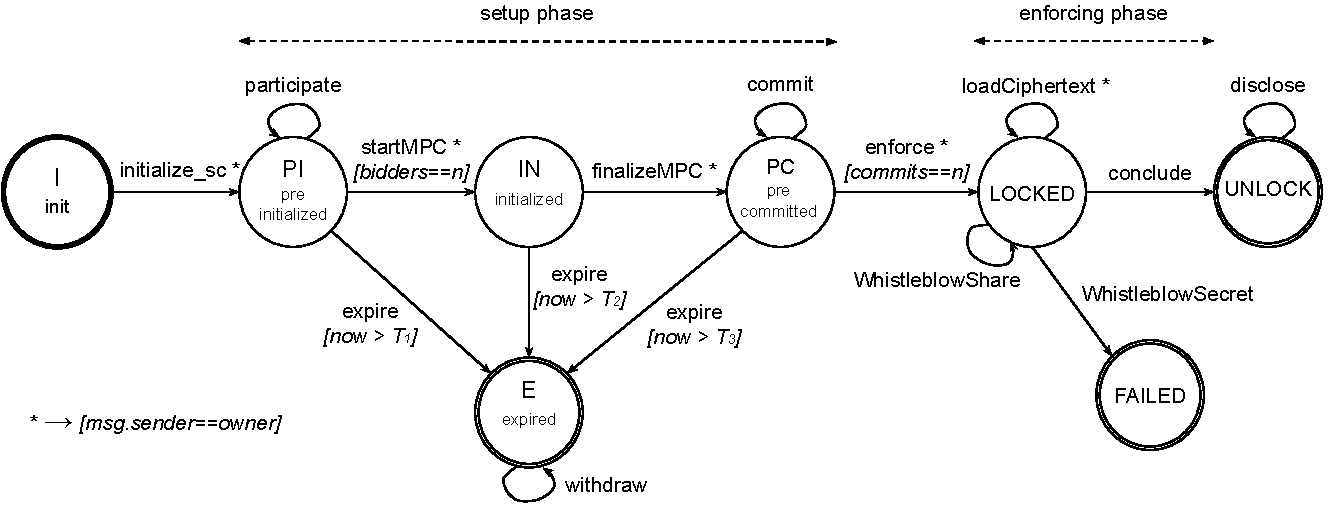
\includegraphics[width=\textwidth]{fig/protocol_fsm_simple_version.pdf}
	\caption{State machine representing the evolution of \shortname protocol. Each transition name maps to an action (an Ethereum smart contract function) that can be called by each participant in order to modify the state. Square brackets contain additional conditions to be met to make valid transitions.}
	\label{fig:fsm}
\end{figure*}

\subsection{\shortname detailed implementation}\label{sect:ityt_exec}
 
To take into account the issues discussed, we designed \shortname protocol as a state machine implemented in an Ethereum smart contract. The state of each instance can be evolved by performing some actions, each action maps to a specific smart contract function that when executed, produces a transaction that is spread across the whole blockchain and validated by all its nodes.

A simplified version of the state machine mentioned (see Figure~\ref{fig:fsm}) is characterized by two phases: a \texttt{setup} phase, in which the owner and the shareholders have to cooperate in order to deploy, configure and activate one instance of the protocol, and an \texttt{enforcing} phase, in which the participants comply with the constraints of the contract and thus effectively realizing the TL primitive as a consequence.

%Furthermore, before participating to a specific instance, each candidate can verify the algorithmic code contained inside the contract. 
%
To make the discussion more clear we point out that the \texttt{setup} phase involves performing {\em off-chain} operations (i.e., all the ones that are not directly performed on the blockchain), therefore it can also be divided in two steps: {\em deployment} and {\em activation}. In between the last two steps the sMPC protocol is executed off-chain by all the participants, its output are the data needed to terminate the configuration of the contract.

The following to illustrate in detail all the execution phases, please refer to Figure~\ref{fig:fsm} for all state and transitions mentioned. 

\medskip

\paragraph*{Setup phase I - deployment}
Initially, the owner deploys an instance of \shortname on the Ethereum blockchain. 
By calling the function \texttt{initialise}, she sends to the contract the pawn, $\PO$, and she is then able to specify: the information about participants, the economic conditions and the time thresholds required for the desired execution; thus landing the protocol to the \texttt{pre initialised} state. 
To demonstrate the will to correctly participating, each shareholder calls the smart contract function \texttt{deposit} and transfers to the contract the proper amount of Ether corresponding to the bid, $B_{\mathcal{H}}$. 
The owner observes the actions taken by all the participants by reading the state of the contract and, after she notices all the shareholders have asserted on the continuation, she then writes on the blockchain the \texttt{initialised} state by calling the function \texttt{startMPC}. The latter action permits to open the sMPC time window, in which all the participants cooperate to bring to completion the sMPC protocol. Its entire execution takes place off-chain, specifically, in the form of a network computation protocol.

\medskip

\paragraph*{sMPC execution}\label{sect:impl_mpc_brief}
We use the sMPC protocol as a tamper proof primitive which permits to securely generate a set of $n$ shares $\left\lbrace \share _0 , \ldots , \share_{n-1} 	\right\rbrace$ of a random key, $\key$. Specifically, the shares are derived from the key using the Shamir's Secret Sharing algorithm~\cite{Shamir:1979:SS:359168.359176}, so that it is possible to reconsruct $\key$ out of {\em k-of-n} shares.
Given the presence of key, we introduce a slight change of notation to make the exposition more clear. 
Specifically, we will use the term plaintext, \plaintext, as an alias for the secret, \secret. 
Given a key, \key, and an encryption algorithm, $\cipvocabulary$, an owner can encrypt a plaintext, \plaintext by performing \wrap, thus obtaining the ciphertext, \ciphertext. 
The advantage of using a key is that it permits to avoid the exposition of \plaintext (the secret), until the current \shortname instance has been activated (see Figure~\ref{fig:key_delayed_wrap}). Other useful implications will be explained in the \texttt{enforcing} phase. \\
...
(see Figure~\ref{fig:mpc1}).
... \\
Before introducing the {\em activation} step of \texttt{setup} phase, we briefly remind that the sMPC permits keeping the input and output of each participant private, thus guaranteeing to each shareholder that no one, except herself, will be able to submit her share at disclosure time. 
The use of an sMPC is then fundamental to guarantee the economic game conditions over which our analysis is based. Further important implications about the use of an sMPC will be discussed later, in Subsection~\ref{sect:impl_mpc}.

\medskip

\paragraph*{Setup phase II - activation}
When the sMPC terminates, all the parties have the data required to properly execute an instance of \shortname. 
Hence, all the participants undergo to the activation procedure of the smart contract. 
To accomplish that, the owner calls the function \texttt{finalizeMPC} and sends to the contract the commitment of the key, $ \commitment _\key $, along with the commitments of all the shares, $\{ \commitment _i , ... , \commitment _n \}$. 
As a consequence, the state of \shortname turns to \texttt{pre committed}. 
Each shareholder is now asked to verify the correctness of the data deposited in the contract by $\owner$. 
In particular, if the commitment written by the owner matched the one given by the shareholder (the owner didn't tampered $\commitment_i$), then each shareholder would perform a \texttt{commit}. 
After each of them committed, the owner invokes \texttt{enforce} and thus she activates the current instance of \shortname (i.e., activation of all economic incentives and penalties). 
The state turns to \texttt{LOCK}, and \texttt{setup} phase ends. 

\medskip

\paragraph*{Enforcing phase}\label{sect:impl_enf_brief}
Once an instance of \shortname reaches the state \texttt{LOCK}, then the TL primitive is active. 

If no adversarial coalition will reconstructs \key before the disclosure time \td, then anyone will be able to call the function \texttt{conclude} to terminate the protocol (\texttt{UNLOCK} state).
All the shareholders will then disclose their share by invoking the function \texttt{disclose}, and each reward will be payed if and only if the share will be  considered valid (i.e., it matches with its correspondent commitment).

Alternatively, the possession of \key demonstrates either its mismanagement by the owner or the collusion among the shareholders; in this setting it is impossible to discriminate between them.   
In fact, anyone in possession of a $\key \sp{\prime} $ can proceed with its submission to the contract by calling the function \texttt{whistleblow}. 
Before transferring to the whistleblower its bonus, \Wsecret, a check for equality between  $\commitment _ { \key \sp{\prime} } $ and $\commitment _ \key $ (i.e., the commitment) is performed. 
If that was the case, the protocol would reach the final state \texttt{FAIL} and consequently all the remaining money locked by the contract would be burned.

We remark that there is no need for the implementation of secret reconstruction function, as all the valid shares will be permanently and publicly be stored on the blockchain: anyone interested in the secret will be able to extract the \key (i.e., by applying Shamir's Secret Sharing algorithm) and then recover the plaintext loaded by the owner by performing the decryption operation, \plaintext $=$ \unwrap. 

The careful reader will have noticed that no mention about sending the ciphertext, \ciphertext, to the contract was made so far. 
Indeed, uploading \ciphertext into the smart contract is (counter-intuitively) optional, as the current implementation is totally agnostic to the presence of \ciphertext or to the meaning of \plaintext. 
The explanation is simple: the outcome of \shortname is only bounded to the disclosure of the key, to which all the incentive and penalties are related to. 
Accordingly, as soon as the state of \shortname takes the value \texttt{LOCK}, before going offline, the owner can opt for uploading \ciphertext into the contract. 
To do that it is only required to wrap the \plaintext by the selected encryption algorithm as shown in~\ref{sect:impl_mpc_brief}, and then to invoke \texttt{loadPlaintext}.

\begin{figure}[t]
	\centering
	\subfloat[A colluding coalition could reveal \secret before contract activation] {{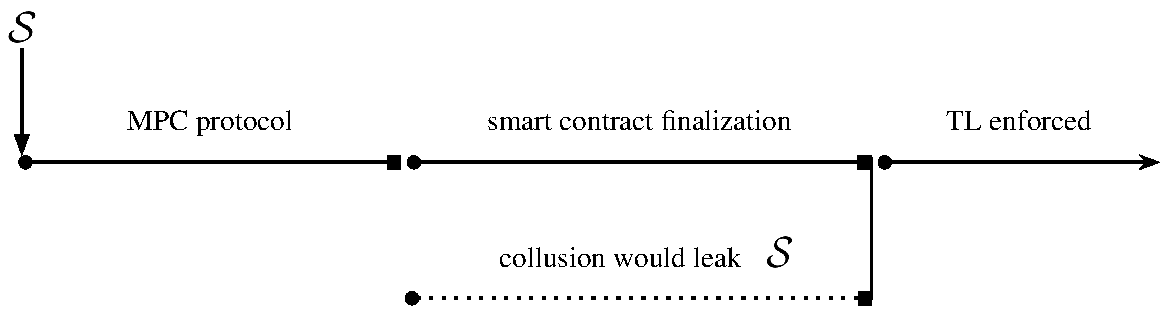
\includegraphics[width=.75\columnwidth]{fig/time1} }}\\
	\vspace*{2pt}
	\subfloat[A colluding coalition could only reveal \key before contract activation] {{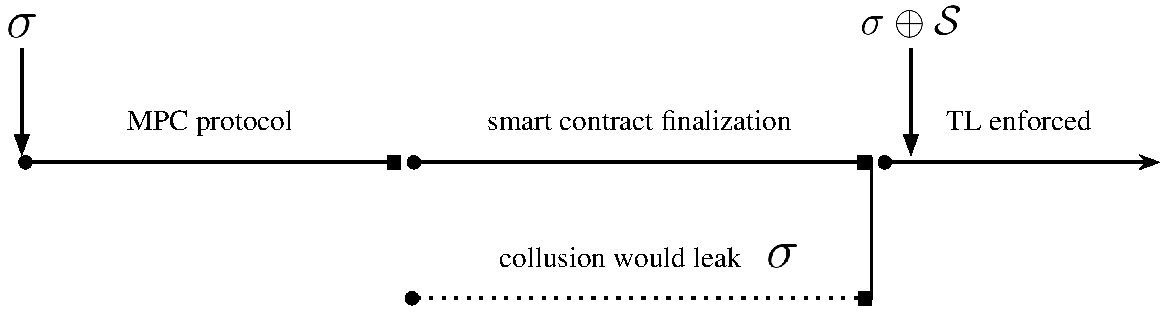
\includegraphics[width=.75\columnwidth]{fig/time2} }}
	\caption{Preventing secret exposure before smart contract activation.}%
	\label{fig:key_delayed_wrap}%
\end{figure}

\begin{figure}[t]
	\centering
	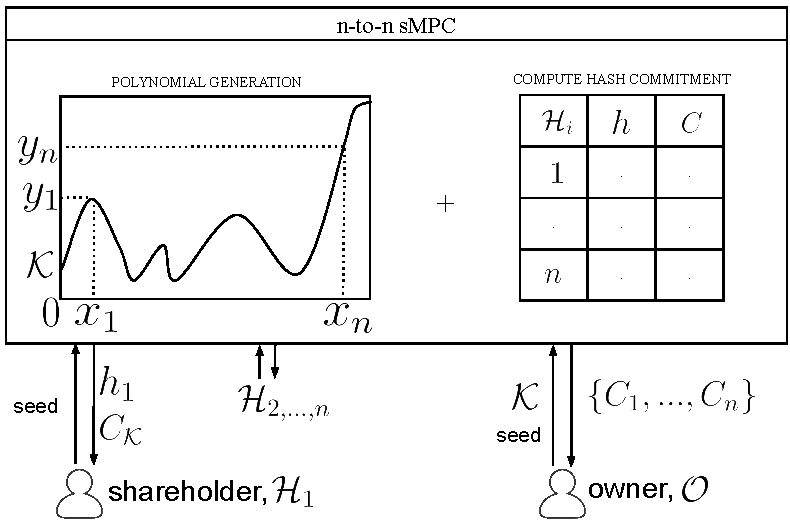
\includegraphics[width=0.75\columnwidth]{fig/mpc_rev_1.pdf}
	\caption{Single-phase sMPC protocol jointly executed by all the participants.}
	\label{fig:mpc1}
\end{figure}


%cost table
\begin{figure}[t]
	\centering
	%\subfloat[Total \shortname gas cost]{
		\begin{tabular}[b]{| c | c | c | c | }	
			\hline
			$n$ &	Owner & Active shareholder & Passive shareholder
			\\	\hline \hline
			2&	6.81 \$&	2.01 \$&	1.10 \$
			\\	\hline
			3&	7.21 \$&	2.03 \$&	1.06 \$
			\\	\hline
			4&	7.60 \$&	2.04 \$&	1.13 \$
			\\	\hline
			5&	8.00 \$&	2.06 \$&	1.14 \$
			\\	\hline
			6&	8.39 \$&	2.07 \$&	1.16 \$
			\\	\hline
			7&	8.79 \$&	2.08 \$&	1.17 \$
			\\	\hline
			8&	9.18 \$&	2.10 \$&	1.19 \$
			\\	\hline
			9&	9.58 \$&	2.11 \$&	1.20 \$
			\\	\hline
			10&	9.97 \$&	2.12 \$&	1.21 \$
			\\	\hline
			
		\end{tabular}
	%}
	%\hfill
	\begin{comment}
	%cost growth
	\subfloat[\shortname linear cost in the number of participants]{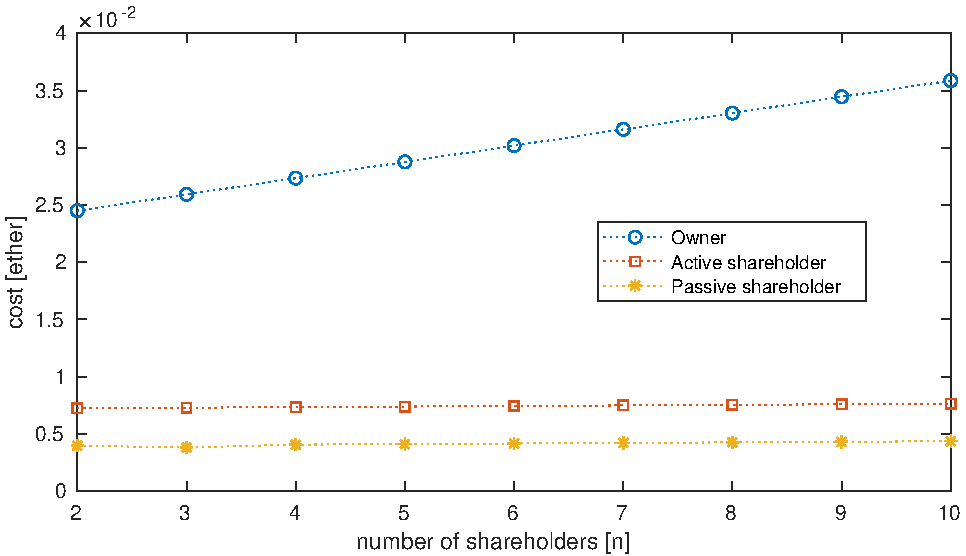
\includegraphics[height=135pt]{ityt_cost_in_ether.pdf}}
	\end{comment}
	\caption{\shortname smart contract gas cost for each role (1 ETH $=$ 221.22 USD)}	
	\label{fig:costfigs}	
\end{figure}
